\documentclass[border=10pt]{standalone}
\usepackage{tikz}\usepackage{amsmath}\usetikzlibrary{calc,arrows.meta}
\begin{document}
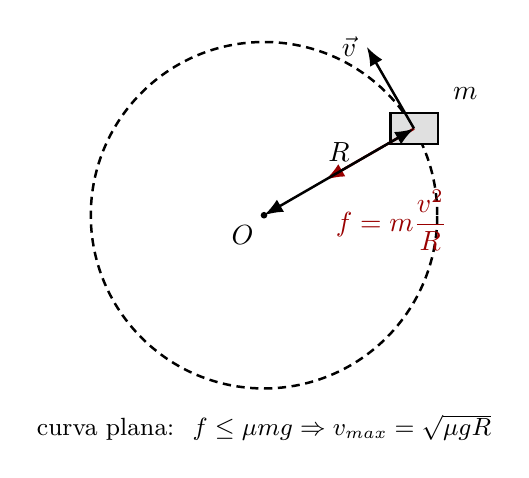
\begin{tikzpicture}[line width=0.9pt,>={Latex[length=2.4mm]}]
  % vista superior: trayectoria circular
  \draw[densely dashed] (0,0) circle(2.2);
  \fill (0,0) circle(1.2pt) node[below left]{$O$};
  \coordinate (P) at (30:2.2);
  \draw[thick,fill=black!12] ($(P)+(-0.3,-0.2)$) rectangle ++(0.6,0.4);
  \node at ($(P)+(0.65,0.45)$){$m$};
  % fuerza de rozamiento hacia el centro
  \draw[->,red!60!black] (P)--($(P)+(210:1.3)$) node[below right]{$f=m\dfrac{v^2}{R}$};
  % velocidad tangente
  \draw[->] (P)--($(P)+(120:1.2)$) node[left]{$\vec v$};
  \draw[<->] (0,0)--(P) node[midway,above]{$R$};
  \node at (0,-2.7){\small curva plana: $\;f\le\mu mg\Rightarrow v_{max}=\sqrt{\mu g R}$};
\end{tikzpicture}
\end{document}
